\documentclass[12pt, french]{report}

\usepackage[top=3cm, bottom=3cm, left=3cm, right=3cm]{geometry}
\usepackage[T1]{fontenc}
\usepackage[utf8]{inputenc}
\usepackage{babel}
\usepackage{graphicx}
\usepackage{hyperref}
\usepackage{pdfpages}
\usepackage{gensymb}
\usepackage{eurosym}
\usepackage{xcolor}
\usepackage{appendix}
\usepackage{amsmath,amsfonts,amssymb}

\hypersetup{                    % parametrage des hyperliens
    colorlinks=true,                % colorise les liens
    breaklinks=true,                % permet les retours à la ligne pour les liens trop longs
    urlcolor= blue,                 % couleur des hyperliens
    linkcolor= blue,                % couleur des liens internes aux documents (index, figures, tableaux, equations,...)
    citecolor= green                % couleur des liens vers les references bibliographiques
    }
   
\begin{titlepage}
\title{	
\includegraphics[scale=0.4]{assets/img/logo-adaltas.png}\\[1 cm]
		\normalsize \textsc{Rapport de stage}\\[0.8cm]
		{Entreprise partenaire : \\Adaltas}\\[0.8 cm]
		\rule{\linewidth}{0.2 mm} \\[0.4 cm]
		\LARGE \textbf{\uppercase{Mise en place d'une solution d'automatisation pour le déploiement de sysèmes Big Data}}
		\rule{\linewidth}{0.2 mm}
		}
\author {\normalsize Auteur :\\	\normalsize Alexander Hoffmann - alexander@adaltas.com\\[0.5 cm]
		 \normalsize Maître de stage :\\	\normalsize David Worms - david@adaltas.com\\}
\date{\normalsize \today}
\end{titlepage}

\begin{document}
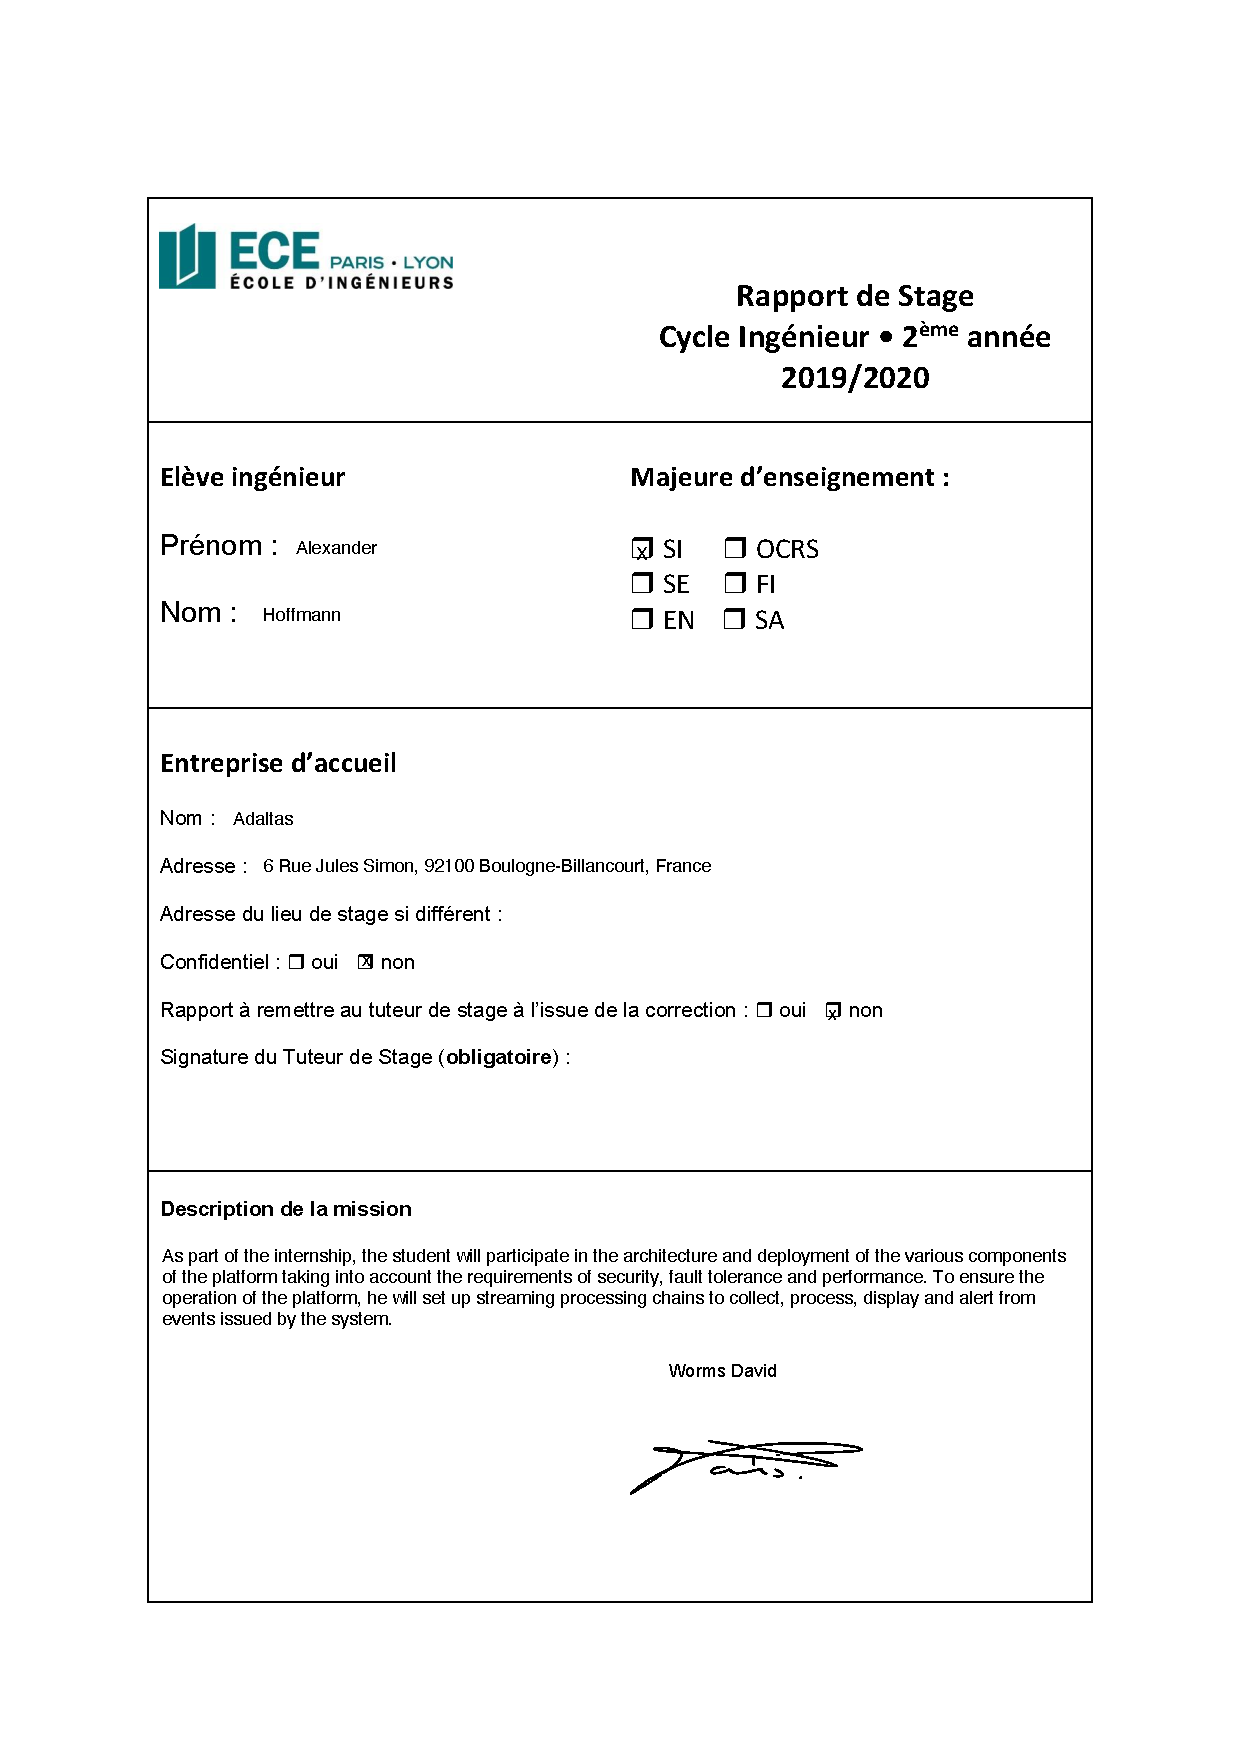
\includepdf[pages=-]{assets/pdf/title.pdf}

\maketitle

\chapter*{Remerciements}

Je tiens tout d’abord à remercier toute l'équipe d'Adaltas pour son accueil, sa bienveillance et sa bonne
humeur permanente.\\

Je voudrais ensuite exprimer ma sincère gratitude à David Worms, mon tuteur, pour la confiance qu’il a bien voulu m’accorder en acceptant de m'intégrer à Adaltas. Je le remercie pour sa grande disponibilité, sa patience, son soutien chaleureux et ses conseils avisés. Je tiens à lui exprimer ma profonde reconnaissance pour ses critiques constructives d’une rigueur absolue.\\

Mes remerciements s’adressent également à Prisca Borges pour son accueil, sa sympathie et ses conseils, ainsi qu'à Léo Schoukroun pour son encadrement et sa compréhension qu'il m'a accordé tout au long du stage.\\

En cette période inédite de crise sanitaire, j'ai eu la chance de pouvoir travailler avec une entreprise qui a su s'adapter aux difficultés posées par les mesures nécessaires à la protection de ses collaborateurs. Je suis reconnaissant d'avoir pu effectuer mon stage dans les meilleurs conditions possibles.

\chapter*{Résumé}

J'ai effectué mon stage de 2ème année du cycle ingénieur au sein de l'entreprise Adaltas. Adaltas est une équipe de consultants experts en Open Source, Big Data et systèmes distribués. La société fournit à ses clients un savoir faire reconnu sur la manière d'utiliser les technologies pour convertir leurs cas d'usage en projets exploités en production, sur la façon de réduire les coûts et d'accélérer les livraisons de nouvelles fonctionnalités.\\

Au sein de cette structure, j'ai eu la chance d'évoluer en tant que développeur. J'ai travaillé sur Nikita, une librairie d’automatisation pour le déploiement de systèmes pour Node.js. Ce logiciel a été conçu dans le but d'aider les développeurs et les opérateurs à déployer des infrastructures et des logiciels Big Data de manière flexible et idempotente.\\

\begingroup
\hypersetup{linkcolor=black}
\tableofcontents
\listoffigures
\newpage
\endgroup

\chapter*{Introduction}
\addcontentsline{toc}{chapter}{Introduction}

\end{document}
